\documentclass[fleqn]{article}

\usepackage[utf8]{inputenc}
\usepackage{graphicx}
\usepackage{amsmath}
\usepackage{tikz}

\newcommand*\circled[1]{\tikz[baseline=(char.base)]{
            \node[shape=circle,draw,inner sep=2pt] (char) {#1};}}

\setlength{\mathindent}{1cm}

\title{Akdemy}
\author{Gabriel Garcia}

\begin{document}
	\maketitle
	\newpage
	\section{Alphabet and Lexem Formation Pattern}
		\begin{figure}[ht!]
			\centering
			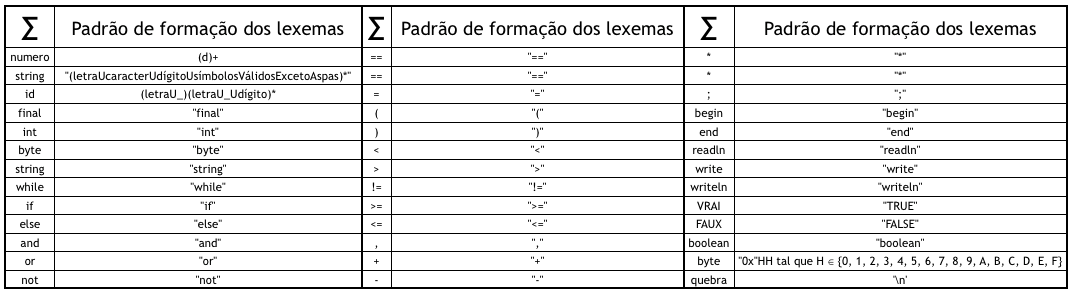
\includegraphics[scale=.4]{alphabet.png}
			\caption{Alphabet and Lexem Formation Pattern}
		\end{figure}
	\newpage
	\section{Lexical Analyser Automata}
		\begin{figure}[ht!]
			\centering
			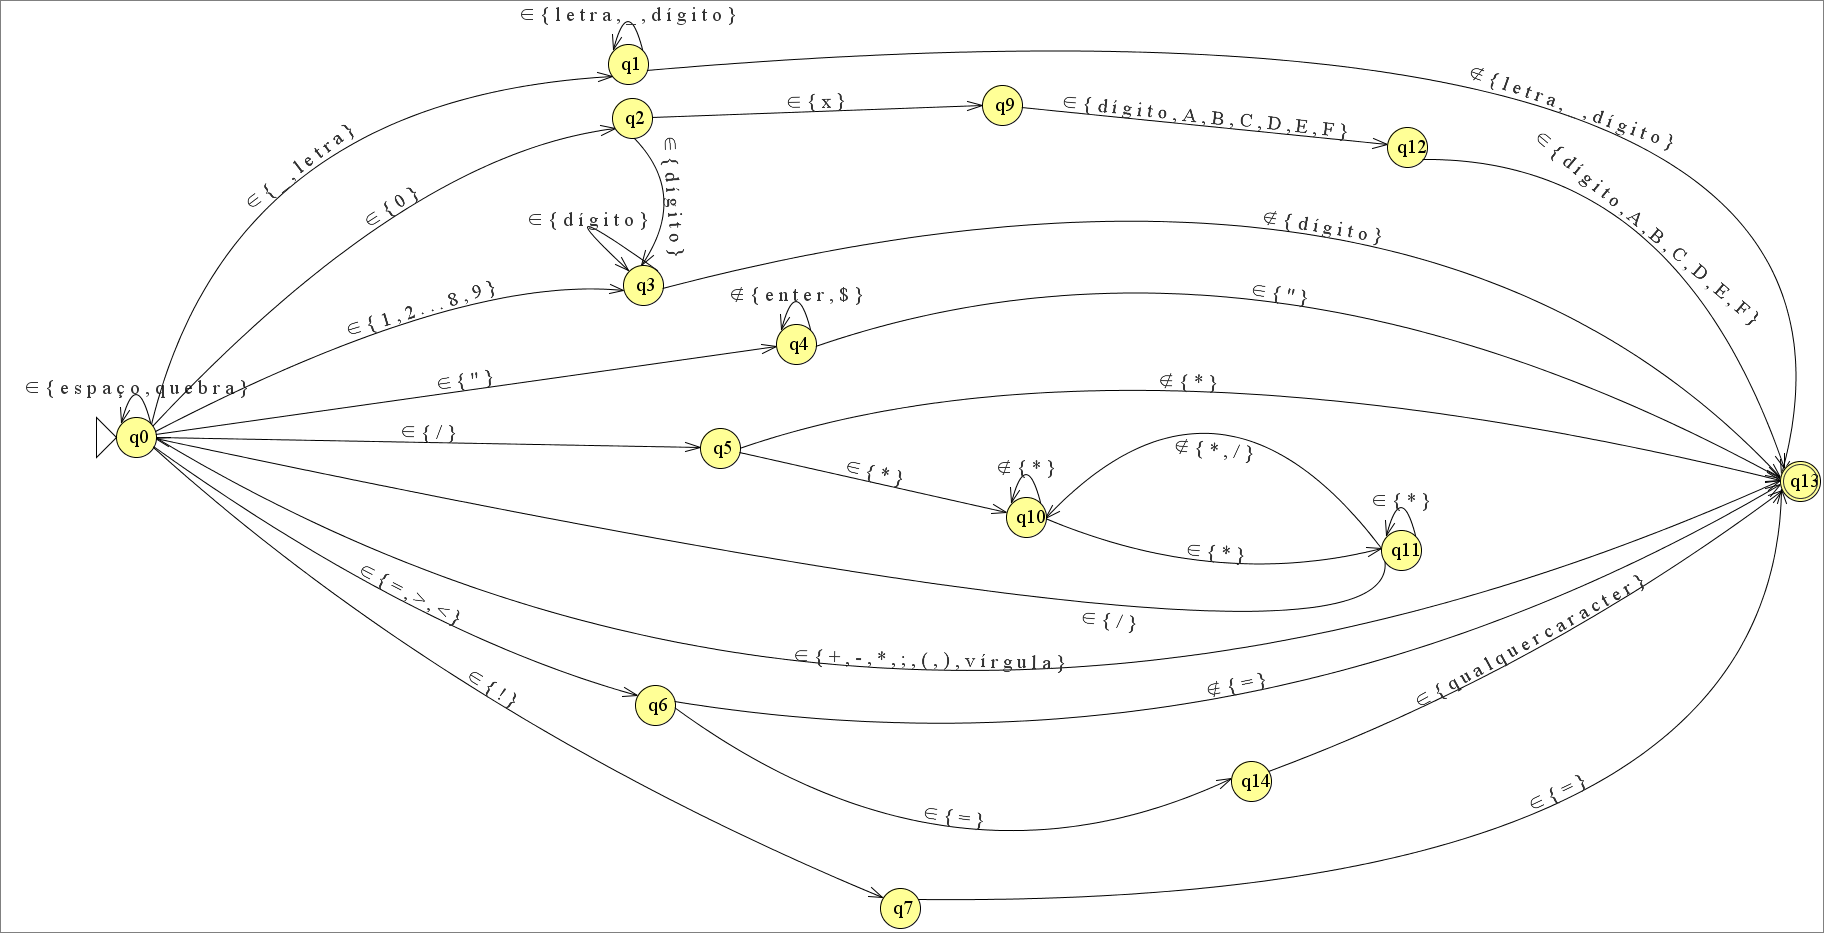
\includegraphics[scale=.26]{automata.png}
			\caption{Lexical Analyser Automata}
		\end{figure}
	\newpage
	\section{Grammar}
		\[ S \rightarrow \circled{1} \circled{2} \{ \circled{3} D \circled{4} \}* \circled{5} \circled{6} B \circled{7} \]
		\[ D \rightarrow (\text{int} \circled{8} |\text{byte}\circled{9}|\text{boolean}\circled{10}|\text{string}\circled{11}) \text{id} \circled{12} \circled{13} \circled{14} [=[(+\circled{15}|-\circled{16})]\circled{17}\text{const}\circled{18} \circled{19}] \]
		\[ \{, \text{id} \circled{12} \circled{13} \circled{14} [=[(+\circled{15}|-\circled{16})]\circled{17}\text{const}\circled{18} \circled{19}]\}*; \]
		\[ D \rightarrow \text{final} ~ \text{id} \circled{20} = [(+\circled{15}|-\circled{16})]\text{const}\circled{21}\circled{22}\circled{23}\circled{24}\circled{25} \]
		\[ B \rightarrow \text{begin} \{C\}* \text{end} \]
		\[ C \rightarrow \text{id}\circled{26}=E; \circled{27} \]
		\[ C \rightarrow \text{while} ~ \circled{28} E \circled{29} \circled{30} (C|B) \circled{31} \]
		\[ C \rightarrow \text{if} ~ E \circled{32} \circled{33} (C|B) \circled{34} [\textit{else}~(C|B)] \circled{35} \]
		\[ C \rightarrow ; \]
		\[ C \rightarrow \text{readln} ~ \text{id}; \circled{36} \circled{37} \]
		\[ C \rightarrow \text{write} ~ E\circled{38}\{,E\circled{39}\}*; \]
		\[ C \rightarrow \text{writeln} ~ E\circled{38}\{,E\circled{39}\}*;\circled{40} \]
		\[ E \rightarrow F\circled{41}[(<\circled{42}|>\circled{43}|<=\circled{44}|>=\circled{45}|==\circled{46}|!=\circled{47}) F\circled{48}] \]
		\[ F \rightarrow [(+\circled{49}|-\circled{50})]G\circled{51}\{(+\circled{52}|-\circled{53}|\text{or}\circled{54})G\}* \]
		\[ G \rightarrow H\circled{55}\{(*\circled{56}|/\circled{57}|and\circled{58})H\circled{59}\}* \]
		\[ H \rightarrow [\circled{60}not]J\circled{61} \]
		\[ J \rightarrow ``("E``)" \]
		\[ J \rightarrow \text{const} \circled{62} \]
		\[ J \rightarrow \text{id} \circled{63} \]

		\begin{itemize}
			\item \circled{1} \{ ``sseg SEGMENT STACK\\\\byte 4000h DUP(?)\\sseg ENDS\\\\dseg SEGMENT PUBLIC\\\\byte 4000h DUP(?)\\" \}
			\item \circled{2} \{ S.addr = 0x4000 \}
			\item \circled{3} \{ D.addr = S.addr \}
			\item \circled{4} \{ S.addr = D.addr \}
			\item \circled{5} \{ ``dseg ENDS\\\\cseg SEGMENT PUBLIC\\ASSUME CS:cseg, DS:dseg\\\\strt:\\" \}
			\item \circled{6} \{ S.attrs \}
			\item \circled{7} \{ ``mov ah, 4Ch\\int 21h\\cseg ENDS\\END strt" \}
			\item \circled{8} \{ D.t = inteiro \\ D.addr += 2 \}
			\item \circled{9} \{ D.t = byte \\ D.addr++ \}
			\item \circled{10} \{ D.t = booleano \\ D.addr++ \}
			\item \circled{11} \{ D.t = string \\ D.addr += 0x100 \}
			\item \circled{12} \{ se id.classe != vazio então \\ id.classe = ``variavel" \\ senão \\ erro(``identificador ja declarado") \}
			\item \circled{13} \{ id.addr = D.addr \}
			\item \circled{14} \{ se D.t == byte ou D.t == booleano \\ S.addr++ \\ se não se D.t == inteiro \\ S.addr += 2 \\ se não se D.t == string \\ S.addr += 0x100 \\ fim se \}
			\item \circled{15} \{ D.s = ``-" \}
			\item \circled{16} \{ D.s = ``+" \}
			\item \circled{17} \{ se D.s == ``-" ou D.s == ``+" então \\ se id.tipo != byte ou id.tipo != inteiro então \\ erro(``tipos incompatíveis") \\ fim se \\ se id.tipo == byte e D.s == ``-" então \\ id.tipo = inteiro \\ fim se \\ fim se \}
			\item \circled{18} \{ se não (id.tipo == const.tipo ou (id.tipo == inteiro e const == byte)) então \\ erro(``tipos incompatíveis") \\ fim se  \}
			\item \circled{19} \{ se id.tipo == string então \\ S.attrs += ``mov bx, id.addr" \\ para cada caractere na string const.lexema faça \\ S.attrs += ``mov al, caractere" \\ S.attrs += ``mov DS:[bx], al" \\ S.attrs += ``add bx, 1" \\ fim para cada \\ S.attrs += ``mov al, 24h" \\ S.attrs += ``mov DS:[bx], al" \\ se não se id.tipo == inteiro então \\ S.attrs += ``mov ax, D.s+const.lexema"\\ S.attrs += ``mov DS:[id.addr], ax" \\ se não se id.tipo == byte então \\ S.attrs += ``mov al, const.lexema" \\ S.attrs += ``mov DS:[id.addr], al" \\ se não se id.tipo == booleano então \\ S.attrs += ``mov al, (const.lexema == TRUE ? FFh : 00h)" \\ S.attrs += ``mov DS:[id.addr], al" \\ fim se \}
			\item \circled{20} \{ se id.classe != vazio então \\ id.classe = ``constante" \\ senão \\ erro(``identificador ja declarado") \}
			\item \circled{21} \{ se D.s == ``-" ou D.s == ``+" então \\ se const.tipo != byte ou const.tipo != inteiro então \\ erro(``tipos incompatíveis") \\ fim se \\ se const.tipo == byte e D.s == ``-" então \\ const.tipo = inteiro \\ fim se \\ fim se \}
			\item \circled{22} \{ id.tipo = const.tipo \\ id.addr = D.addr \}
			\item \circled{23} \{ se const.tipo == string então \\  \}
			\item \circled{24} \{ se D.t == byte ou D.t == booleano \\ S.addr++ \\ se não se D.t == inteiro \\ S.addr += 2 \\ se não se D.t == string \\ S.addr += strlen(const.lexema) \\ fim se \}
			\item \circled{25} \{ se id.tipo == string então \\ ``byte const.lexema\$" \\ se não se id.tipo == byte então \\ ``byte const.lexema" \\ se não se id.tipo == booleano então \\ ``byte (const.lexema == TRUE ? FFh : 00h)" \\ se não \\ ``sword D.s+const.lexema" \\ fim se \}
			\item \circled{26} \{ se id.classe == vazio então \\ erro(``identificador nao declarado") \\ se não se id.classe == constante então \\ erro(``classe de identificador incompativel") \\ fim se \}
			\item \circled{27} \{ se id.tipo == inteiro então \\ se E.tipo == inteiro então \\ ``mov al, DS:[E.addr]" \\ ``mov al, DS:[E.addr+1]" \\ ``mov DS:[id.addr], al" \\ ``mov DS:[id.addr+1], ah" \\ se não \\``mov al, DS:[E.addr]" \\ ``mov ah, 0" \\ ``mov DS:[id.addr], al" \\ ``mov DS:[id.addr+1], ah" \\ fim se \\ se não se id.tipo == string então \\ ``mov bx, E.addr" \\ ``mov di, id.addr" \\ loop = NovoRot \\ end = NovoRot \\ ``loop:" \\ ``mov cl, DS:[bx]" \\ ``cmp cl, 24h" \\ ``je end" \\ ``mov DS:[di], cl" \\ ``add di, 1" \\ ``add bx, 1" \\ ``jmp loop" \\ ``end:" \\ ``mov DS:[di], cl" \\ se não \\ ``mov al, DS:[E.addr]" \\ ``mov DS:[id.addr], al" \\ fim se  \}
			\item \circled{28} \{ loop = NovoRot \\ end = NovoRot \\ ``loop:" \}
			\item \circled{29} \{ se E.tipo != booleano então erro(``tipos incompatíveis.") fim se \}
			\item \circled{30} \{ ``mov al, DS:[E.addr]" \\ ``mov ah, 0" \\ ``cmp ax, 0" \\ ``je end" \}
			\item \circled{31} \{ ``jmp loop" \\ ``end: " \}
			\item \circled{32} \{ false = NovoRot \\ end = NovoRot \\ se E.tipo != booleano então erro(``tipos incompatíveis.") fim se \}
			\item \circled{33} \{ ``mov al, DS:[E.addr]" \\ ``mov ah, 0" \\ ``cmp ax, 0" \\ ``je false" \}
			\item \circled{34} \{ ``jmp end" \\ ``false:" \}
			\item \circled{35} \{ ``end:" \}
			\item \circled{36} \{ buffer = NovoTemp \\ ``mov dx, buffer" \\ ``mov al, 0FFh" \\ ``mov DS:[buffer], al" \\ ``mov ah, 0Ah" \\ ``int 21h" \\ ``mov ah, 02H" \\ ``mov dl, 0Dh" \\ ``int 21h" \\ ``mov dl, 0Ah" \\ ``int 21h" \}
			\item \circled{37} \{ end = NovoRot \\ loop = NovoRot \\ se id.tipo == string então \\ ``mov di, id.addr" \\ ``mov bx, buffer+2" \\ ``loop: " \\ ``mov al, DS:[bx]" \\ ``cmp al, 0Dh" \\ ``je end" \\ ``mov DS:[di], al" \\ ``add di, 1" \\ ``add bx, 1" \\ ``jmp loop" \\ ``end:" \\ ``mov al, 24h" \\ ``mov DS:[di], al" \\ se não se id.tipo == byte \\ ``mov di, buffer+2" \\ ``mov al, 0" \\ ``mov cl, 10" \\ ``loop:" \\ ``mov bl, DS:[di]" \\ ``cmp bl, 0Dh" \\ ``je end" \\ ``mul cl" \\ ``add bl, -48" \\ ``add al, bl" \\ ``add di, 1" \\ ``jmp loop" \\ ``end:" \\ ``mov DS:[id.addr], al" se não se id.tipo == inteiro então \\ positive = NovoRot \\ ``mov di, buffer+2" \\ ``mov ax, 10" \\ ``mov cx, 10" \\ ``mov dx, 1" \\ ``mov bl, DS:[di]" \\ `` jne positive" \\ ``mov dx, -1" \\ ``add di, 1" \\ ``mov bl, DS:[di]" \\ ``cmp bl, 0Dh" \\ ``je end" \\ ``imul cx" \\ ``add bl, -48" \\ ``mov bh, 0" \\ ``add ax, bx" \\ ``add di, 1" \\ ``jmp loop" \\ ``end:" \\ ``pop cx" \\ ``imul cx" \\ ``mov DS:[id.addr], al" \\ ``mov DS:[id.addr+1], ah" \}
		\end{itemize}



\end{document}